\chapter{Transferring Files}

\section{Getting Files to the MEGA65}
\label{cha:transferring-files}
\index{SD Cards!Transferring Files}

While there is plenty of fun to be had writing your own programs for the MEGA65, eventually you will want to run programs written by others. You may also want to back up your MEGA65 programs to your PC for safe keeping.

The fastest and most reliable way to transfer files between your PC and your MEGA65 is with an Ethernet cable.\index{Networking!Ethernet} You connect one end of the cable to the RJ45 jack on the rear of the MEGA65. You can connect the other end to your local area network (LAN) router or switch, or connect it directly to your PC. You use software on your PC to initiate file transfers, in either direction: from the PC to the MEGA65, or from the MEGA65 to the PC.

Alternatively, you can copy D81 virtual disk images to your MEGA65-formatted SD card using any PC with an SD card reader, without any other special tools or software. Your PC will recognize the data region of the SD card as a FAT32 partition. If you use this method, be aware that some PC operating systems may have unwanted side effects, such as fragmentation of SD card files, or extraneous files created by macOS Finder. These effects are harmless to the data, but may require maintenance to keep the card useful in the MEGA65. If the MEGA65 reports a fragmented file, you can use a PC disk defragmentation tool on the data partition. Alternatively, you can copy all files off of the SD card to the PC, re-format the SD card in the MEGA65, then copy the files back from the PC.

It is also possible to transfer files using a JTAG or UART Serial interface connected to the main board. This is an advanced technique and is not described in this User's Guide. JTAG or UART Serial hardware provides access to a debugging interface that may be useful to some programmers. JTAG is also useful for developing FPGA cores. For more information, see the {\it MEGA65 Developer's Guide.}

Most people will prefer the Ethernet method. This chapter describes how to do this.

\section{Understanding Networking}

The MEGA65 can use Ethernet to connect to or accept connections from other computers on a network. With appropriate software, it can connect to other computers over the Internet.

The MEGA65 Ethernet hardware presents a Media Access Control (MAC) address to the local network.\index{Networking!MAC address} Unlike other Ethernet hardware, the MEGA65's MAC address is not assigned at the factory: it is set in the Configuration Utility. (See chapter \vref{cha:configuringyourmega}.)

To transfer files, you instruct the MEGA65 to make itself available for incoming connections, then use the M65Connect app (or another tool, such as \texttt{mega65\_ftp}) on your PC to initiate a connection. Your PC's operating system may prompt for permission to grant the tool access to the network when you run it for the first time. The tool uses UDP port 4510 to establish the initial connection with the MEGA65, and uses a self-assigned IPv6 address created from the MEGA65's MAC address for the file transfer session. This requires that IPv6 be enabled on the PC's network interface, which is the default in most cases.

As an alternative to connecting the MEGA65 to your local network, if your PC has an Ethernet jack, you can connect your MEGA65 directly to your PC with an Ethernet cable. This forms a small local network with no access to the Internet. The procedure for transferring files is the same with a direct connection as with a local network connection.

\section{Obtaining M65Connect}
\index{M65Connect Application}

{\bf M65Connect} is an application for Windows, Mac, or Linux that facilitates file transfers and other useful features for MEGA65 users. The application has a windowed interface, and also includes command-line tools useful for programming.

To obtain M65Connect:

\begin{enumerate}
\item Visit the MEGA65 Filehost website\index{Filehost website} in a browser: \url{https://files.mega65.org}
\item In the search box in the top right corner, type: ``M65Connect''
\item Select the version of M65Connect for your PC operating system.
\item Click the ``Download'' button.
\item Use your PC to unpack the downloaded archive file.
\end{enumerate}

\subsection{M65Connect for Windows}

The Windows version of M65Connect is in the ``M65Connect'' folder: {\bf M65Connect.exe}. As with most open source software, Microsoft Defender may refuse to run the software, displaying a dialog window. If this happens, click ``More info,'' then click the ``Run anyway'' button that appears.

The command-line tools are in a sub-folder named ``M65Connect Resources,'' such as: {\tt M65Connect Resources\textbackslash{}mega65\_ftp.exe}

\subsection{M65Connect for macOS}

The macOS version of M65Connect is a Mac application bundle: {\bf M65Connect.app}. As with most open source software, macOS does not recognize it as ``signed'' by the developer, and macOS will refuse to run it. You will need to remove the ``quarantine'' attribute to run the application.

In most versions of macOS, the best way to remove the quarantine attribute is with a Terminal command:

\begin{enumerate}
\item Move the M65Connect app to your Applications folder.
\item Open the Terminal app, included with macOS. This can be found in the Applications folder, in a sub-folder named Utilities.
\item Enter this command: {\tt xattr -cr /Applications/M65Connect.app}
\end{enumerate}

You can now double-click the M65Connect app to run it.

The command-line tools are inside the application bundle directory, such as: {\tt /Applications/M65Connect.app/Contents/Resources/mega65\_ftp.osx}

\subsection{M65Connect for Linux}

The Linux version of M65Connect is in the ``M65Connect'' folder: {\bf M65Connect}. Double-click it to run.

The command-line tools are in a sub-folder named ``M65Connect Resources,'' such as: {\tt M65Connect Resources/mega65\_ftp}

\section{Enabling Network Listening}
\index{Networking!Network Listening Mode}

By default, the MEGA65 ignores all attempts by other computers to connect to it over the network. Software running on the MEGA65 can listen for network connections, but the MEGA65 does not do this on its own.

To transfer files with M65Connect, you must tell the MEGA65 to listen for incoming connection attempts from M65Connect. To enable a network listening session, press \specialkey{SHIFT} + \megakey{\pounds}. The power light blinks between yellow and green when network listening is active.

\begin{center}
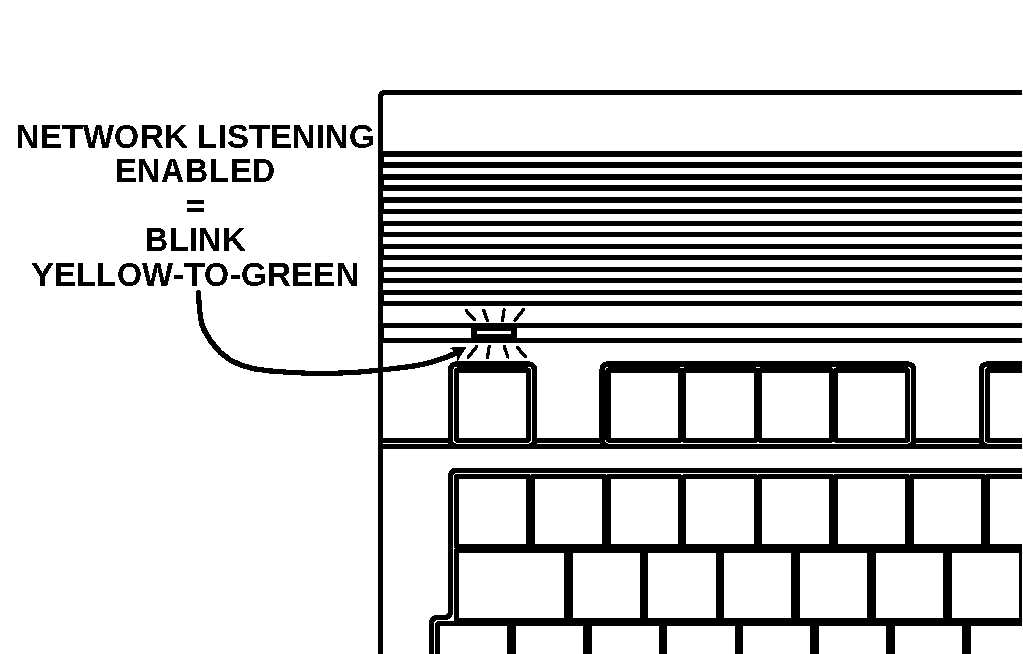
\includegraphics[width=\linewidth]{images/illustrations/mega65-eth-blink.pdf}
\end{center}

To disable network listening, press \specialkey{SHIFT} + \megakey{\pounds} again, or reset the computer.

If the power light does not start blinking after pressing \specialkey{SHIFT} + \megakey{\pounds}, you may need to set DIP switch \#2 on the mainboard. MEGA65s manufactured in the year 2024 and later should have this switch set at the factory. Earlier MEGA65s have this switch off by default.

To set the DIP switch,\index{DIP switches} open the case, as described in chapter \vref{cha:setup}. Locate the DIP switches on the mainboard, then set DIP switch \#2 to the ``on'' position. Look for markings on the switches to identify switch \#2 and the ``on'' direction. (The orientation of your DIP switches may differ from this diagram.)

\begin{center}
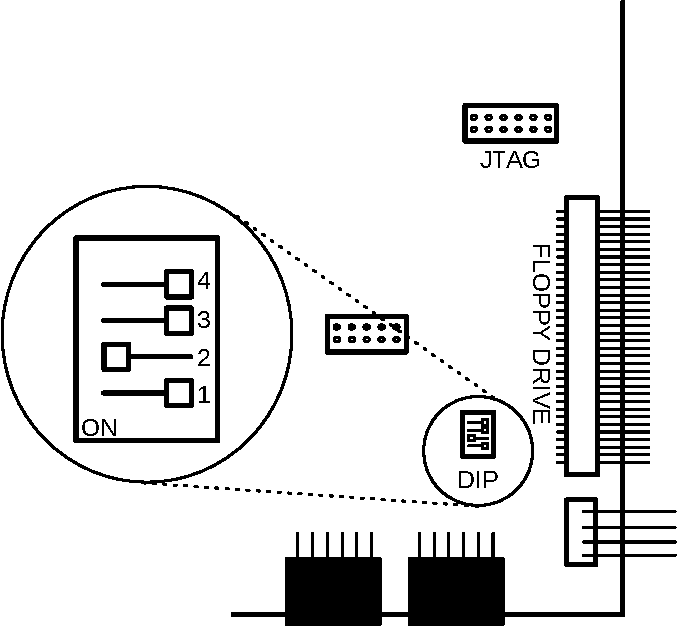
\includegraphics[width=\linewidth]{images/illustrations/mega65-dip2.pdf}
\end{center}

It is safe to leave DIP \#2 in this position for regular operation.


\section{Transferring Files}

To transfer files, you will start a file transfer session using the M65Connect application or the {\tt mega65\_ftp} command-line tool. This connects to the MEGA65 and uploads a file transfer client for use during the session. When you end the session, the MEGA65 resets.

Starting a file transfer session resets the MEGA65. Be sure to save any programs or data before proceeding.

\underline{NOTE}: If you clear memory by resetting the computer, remember to re-enable network listening: press \specialkey{SHIFT} + \megakey{\pounds}, and ensure the power light is blinking.

\subsection{Transferring Files with M65Connect}
\index{M65Connect Application}

M65Connect detects automatically whether the MEGA65 is listening for connections. Open M65Connect, then enable the network listening session on the MEGA65. M65Connect reports a status of "Connected to MEGA65 via LAN," and several buttons including the {\bf PRG} and {\bf SD Card} buttons are enabled in the M65Connect window.

\begin{center}
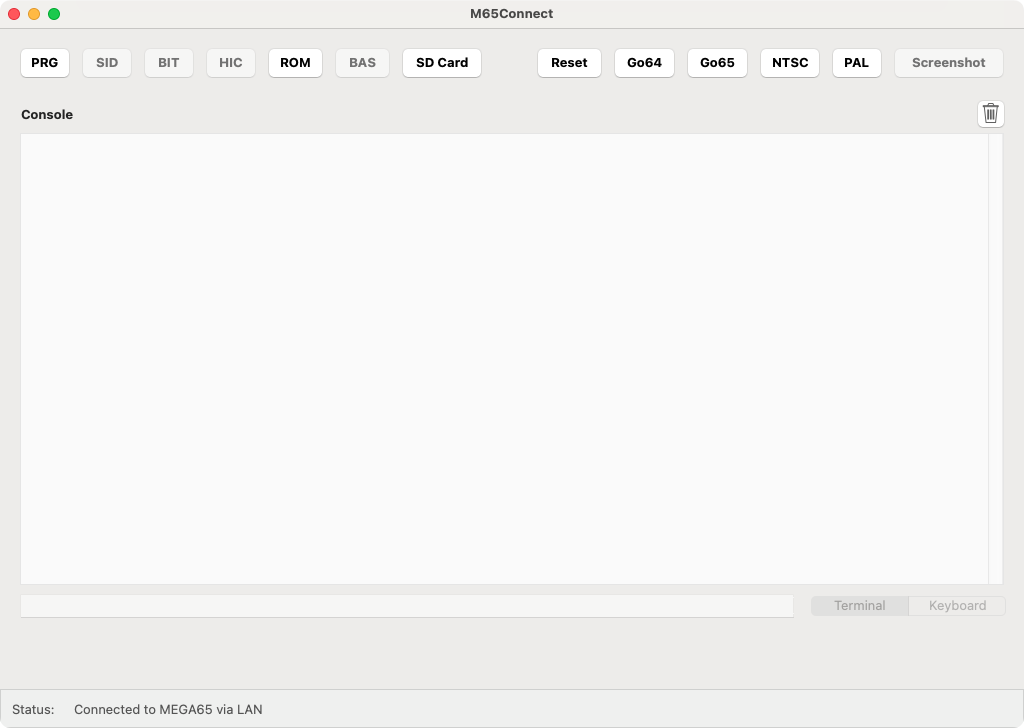
\includegraphics[width=\linewidth]{images/m65connect_macos.png}
\end{center}

If M65Connect reports a status of "Not connected to MEGA65," check the following:

\begin{itemize}
\item The MEGA65 and the PC are connected to the same network, or directly to each other via a network cable.
\item The MEGA65 is in network listening mode, with a blinking power light.
\item In M65Connect, open the Settings menu, and select Connections. The "LAN Port" field should contain an IPv6 address. If it doesn't, wait a few seconds, or click the "Autodetect LAN Port" button.
\end{itemize}

To start a file transfer session, click the {\bf SD Card} button. The SD Card Manager window opens.

\underline{NOTE}: Starting a file transfer session resets the MEGA65 to load the file transfer utility. Be sure to save any data on the MEGA65 before starting the session.

\begin{center}
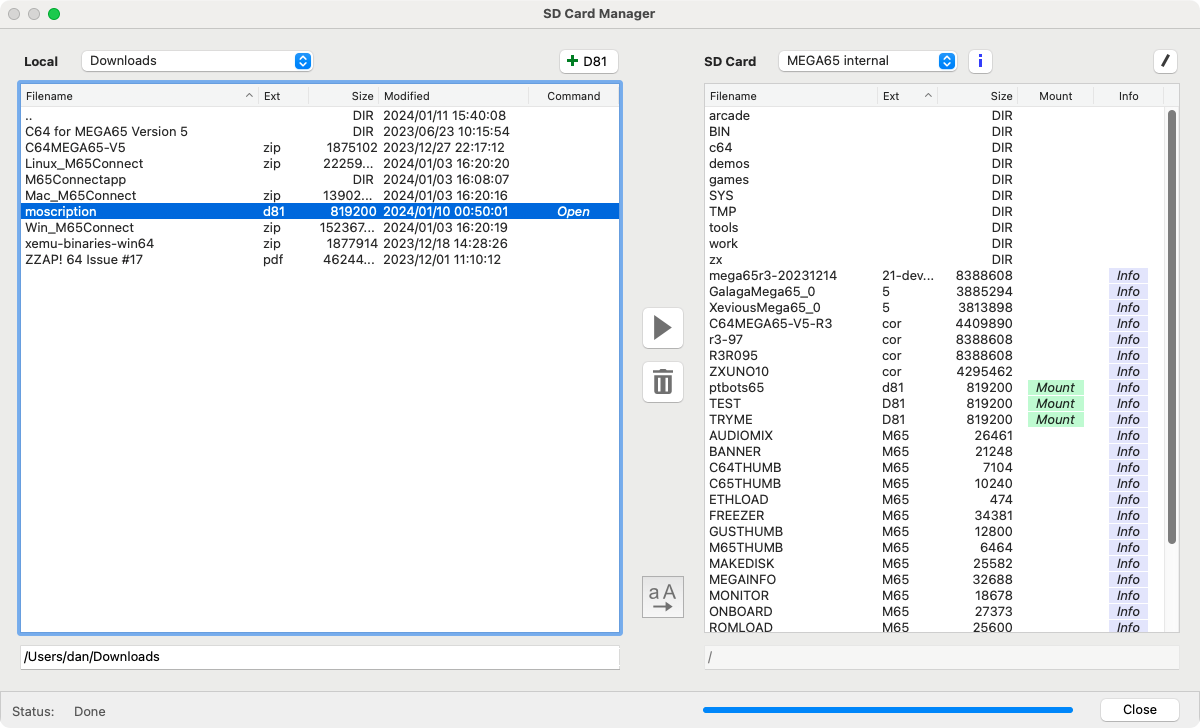
\includegraphics[width=\linewidth]{images/m65connect_files.png}
\end{center}

Use the pane on the left to navigate files on your PC. Use the pane on the right to navigate files on the MEGA65 SD card. To transfer a file, select the file, then click the arrow button. The button indicates the direction the file will transfer.

You can also use M65Connect to create D81 disk images, and copy files to and from D81 disk images. Locate a D81 disk image on your PC or click the {\bf + D81} button to create one, then click the "Open" command in the file browser to open the disk image in the left pane. Transfer files to and from the image with the arrow button. Click the {\bf X} button in the upper right to return to the file browser.

Click the {\bf Close} button to end the file transfer session and close the SD Card Manager window. This resets the MEGA65.

\subsection{The mega65\_ftp Command-Line Tool}
\index{mega65\_ftp command@\texttt{mega65\_ftp command}}

The {\tt mega65\_ftp} command-line tool initiates a file transfer session with the MEGA65. It can run interactively in the terminal and accept multiple file transfer commands, or it can run non-interactively with those commands provided as arguments.

To start an interactive file transfer session, run the {\tt mega65\_ftp} command, providing the {\tt -e} argument to say you want to use an Ethernet connection.

\underline{NOTE}: Starting a file transfer session resets the MEGA65 to load the file transfer utility. Be sure to save any data on the MEGA65 before starting the session.

\begin{verbatim}
% mega65_ftp -e
\end{verbatim}

The tool will upload the file transfer client, and you will see the client running on the MEGA65. If nothing happens, press Ctrl-C (on the PC) to abort, then double-check that the MEGA65 is connected and that network listening is enabled.

Once connected, the file transfer command prompt looks similar to this:

\begin{verbatim}
MEGA65 SD-Card:/>
\end{verbatim}

To end the session, use the {\tt exit} command. The tool will exit and return to the shell prompt, and the MEGA65 will reset.

\begin{verbatim}
MEGA65 SD-Card:/> exit
%
\end{verbatim}

The following are several useful commands you can use during the file transfer session. Use the {\tt help} command to see a complete list of available commands.

\begin{center}
\begin{tabular}{|l|l|}
\hline
{\bf Command} & {\bf Description} \\
\hline
{\tt put {\it filename}} & Send a file from the PC to the MEGA65. \\
\hline
{\tt get {\it filename}} & Retrieve a file from the MEGA65 to the PC. \\
\hline
{\tt dir} & Display a directory listing of the MEGA65 SD card. \\
\hline
{\tt ldir} & Display a directory listing of the local current working directory. \\
\hline
{\tt mkdir {\it dirname}} & Create a sub-directory on the MEGA65 SD card. \\
\hline
{\tt cd {\it dirname}} & Change the current working directory on the MEGA65 SD card. \\
\hline
{\tt lcd {\it dirname}} & Change the local current working directory. \\
\hline
{\tt help} & Display a list of available commands. \\
\hline
{\tt exit} & End the file transfer session. \\
\hline
\end{tabular}
\end{center}

To invoke {\tt mega65\_ftp} commands without starting an interactive prompt, use the {\tt -c} argument once for each command:

\begin{verbatim}
% mega65_ftp -e -c 'put mydisk.d81' -c 'exit'
\end{verbatim}

The tool will start a session, execute the commands, then terminate. Be sure to issue the {\tt exit} command as the final command to reset the MEGA65, or reset the MEGA65 manually after the file transfer has completed.